\section{Test\-Eval Class Reference}
\label{classTestEval}\index{TestEval@{TestEval}}
Inheritance diagram for Test\-Eval::\begin{figure}[H]
\begin{center}
\leavevmode
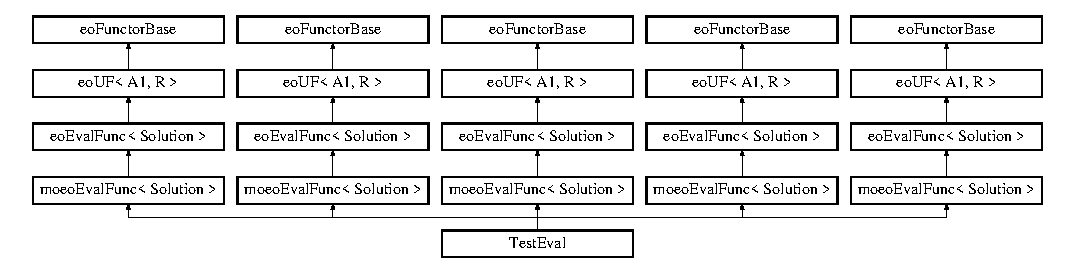
\includegraphics[height=3.23699cm]{classTestEval}
\end{center}
\end{figure}
\subsection*{Public Member Functions}
\begin{CompactItemize}
\item 
void \bf{operator()} (\bf{Solution} \&\_\-sol)\label{classTestEval_9572c868f92fafc149e6da9bcfa7b06b}

\item 
void \bf{operator()} (\bf{Solution} \&\_\-sol)\label{classTestEval_9572c868f92fafc149e6da9bcfa7b06b}

\item 
void \bf{operator()} (\bf{Solution} \&\_\-sol)\label{classTestEval_9572c868f92fafc149e6da9bcfa7b06b}

\item 
void \bf{operator()} (\bf{Solution} \&\_\-sol)\label{classTestEval_9572c868f92fafc149e6da9bcfa7b06b}

\item 
void \bf{operator()} (\bf{Solution} \&\_\-sol)\label{classTestEval_9572c868f92fafc149e6da9bcfa7b06b}

\end{CompactItemize}


\subsection{Detailed Description}




Definition at line 72 of file t-moeo\-Easy\-EA.cpp.

The documentation for this class was generated from the following files:\begin{CompactItemize}
\item 
t-moeo\-Easy\-EA.cpp\item 
t-moeo\-IBEA.cpp\item 
t-moeo\-Max3Obj.cpp\item 
t-moeo\-NSGA.cpp\item 
t-moeo\-NSGAII.cpp\end{CompactItemize}
